\documentclass[11pt,letterpaper]{article}
\usepackage[margin=1in]{geometry}
\usepackage[T1]{fontenc}
\usepackage{lmodern,microtype}
\usepackage{amsmath,amssymb,booktabs,array,longtable,float}
\usepackage{xcolor,hyperref}
\usepackage{tikz}
\usepackage{graphicx}
\graphicspath{{paper/figures/}{figures/}}
\definecolor{navy}{HTML}{17364D}
\definecolor{teal}{HTML}{167D8D}
\hypersetup{colorlinks=true,linkcolor=navy,urlcolor=teal,citecolor=navy,
 pdftitle={From Equity Pairs to Options Relative Value},pdfauthor={Adam Kreitzman and Soo Xin Yang}}
\setlength{\parskip}{0.4em}
\setlength{\parindent}{0pt}
\setlength{\emergencystretch}{2em}
\widowpenalty=10000
\clubpenalty=10000
\renewcommand{\arraystretch}{1.06}
\newcommand{\money}[1]{\$#1}
\title{\textbf{From Equity Pairs to Options Relative Value}\\[0.4em]
\large Does reinforcement learning improve capital allocation?}
\author{Adam Kreitzman and Soo Xin Yang\\MFE 230Z: Deep Learning in Finance}
\date{8 October 2026}
\begin{document}
\maketitle
\begin{abstract}
We adapt equity-pairs trading to relative implied volatility in approximately
30-day, 25-delta out-of-the-money puts on related equity underlyings. First, a
screening rule identifies trade opportunities. Direct policy-search reinforcement
learning (RL) then chooses their entry size, using a decision tree and the
cross-entropy method. We compare this policy with constant full sizing in a
simulated \money{10 million} account over January 2022--August 2025. Annualized
excess Sharpe rises from 1.055 to 1.263, a gain of 0.208 with a conditional
95\% interval of $[-0.103,0.424]$. The learner admits 110 trades; constant full
sizing admits 75. Both produce positive historical profit above cash, and
learned sizing has the higher point estimate. This does not establish a
repeatable advantage: results vary across years, the history was previously
inspected, training and evaluation conventions differ, and execution is simplified.
\end{abstract}

\section{Introduction}
Suppose AMD and NVDA face similar news, but AMD options become unusually expensive
relative to NVDA options. Selling the richer options and buying the cheaper ones
expresses a view about the relative price of volatility. We hedge the stock
exposure daily to reduce immediate directional risk. We also match the legs'
initial vega to reduce sensitivity to a common small change in implied volatility.
These hedges leave other risks. Related stocks can experience different events,
and their option premiums may correctly reflect those differences.

Ning and Lee's equity-pairs framework \cite{ning} separates two decisions:
constructing a spread and learning how to trade it. We use the same distinction
for options. We first ask whether a screened relative-volatility rule produces
useful historical trades under explicit contract and funding assumptions. We
then ask: \emph{does learning improve how capital is allocated to those
opportunities?} Evidence that a signal is profitable does not, by itself,
show that learning improves its allocation.

The report follows that sequence. We explain the motivating paper, define our
option trade, and describe the monthly tree/CEM sizing procedure. We then compare
constant and learned sizing under the same funded-account rules and examine
annual results. The comparison uses the retained configuration and saved
historical backtests.

We measure performance using annualized Sharpe of daily returns above the
cash benchmark, profit above cash and cash-relative drawdown.
Appendix~\ref{app:metrics} defines these measures and records the opening
portfolios at the reporting boundary.

\clearpage
\section{Motivating paper and adaptation}
\subsection*{What the paper does}
Ning and Lee \cite{ning} first construct a mean-reverting equity spread. Let
$S_{1,t}$ and $S_{2,t}$ be the two stock prices at time $t$. Their spread is
$X_t=S_{1,t}-B S_{2,t}$, where $B$ is a hedge coefficient. They choose $B$ by
grid search to minimize empirical mean reversion time: the average time from a
significant local extreme to the next mean crossing. This formation step does
not fit an Ornstein--Uhlenbeck (OU) mean-reversion model.

They then use tabular Q-learning to trade the spread. The state records the
direction and magnitude of recent spread moves. The available actions are to
buy, hold or sell a unit, subject to the current position. The policy opens a
long spread and later closes it; it does not open a short spread. The reward
favors buying below and selling above the equilibrium mean. It also includes
the transaction-cost term $c|A|$, where $c$ is the cost coefficient and $|A|$
the action's magnitude. Q-values combine the immediate reward with the estimated
value of subsequent decisions.

Training precedes the historical market test. Because the reward requires a
true equilibrium mean, the agent trains on 10,000 one-year simulated OU paths.
The market study then forms ten US pairs in 2022 and trades them in 2023. For
all ten pairs, the published daily Sharpe ratios exceed the Distance Method
and OU benchmarks. These daily figures are not directly comparable with our
annualized options Sharpe ratios.

\subsection*{Criticisms that motivate our design}
Three issues limit interpretation. \textbf{Short history:} one trading year
offers little evidence across regimes. \textbf{Costs and scale:} the reward
includes a cost term, but the numerical implementation and reconciliation to
net performance are not clearly documented. That does not show that costs
were omitted. Higher turnover increases total costs, while larger or faster
orders can increase per-unit slippage and market impact. A constant cost
coefficient therefore does not establish scalability. \textbf{Simulation transfer:}
spread formation is empirical, but training assumes specified mean-reverting
dynamics and a known equilibrium. Real relationships can shift; extensive
synthetic experience alone does not establish transfer to markets.

\subsection*{What we borrow and what we change}
We retain the separation of opportunity construction from trading decisions
and ask whether learning improves on a simple rule. Our instrument changes
from equity-price spreads to option-implied-volatility spreads. We use actual
contracts, match initial vega and hedge stock delta daily. For training, we
replace the known synthetic equilibrium with completed historical outcomes.
We also specify simulated costs explicitly and compare multiple trading years.

The next section follows a trade from its relative-IV signal through contract
selection and hedging to expiry. We then explain how a regression tree groups
completed historical opportunities. Direct policy-search RL uses the
cross-entropy method (CEM) to choose an entry size for each group. The comparison
with constant sizing measures the additional historical value of learned allocation.

\clearpage
\section{Our strategy and evaluation}
\subsection{From a volatility signal to a hedged trade}
Implied volatility (IV) is the volatility that reproduces an option quote under
a pricing model. Realized volatility (RV) measures stock-price variation; our
RV inputs use only trailing data available at the signal date. We trade puts
near 25 delta and 30 days to expiry (P25), with strikes below the stock price.
At delta $-0.25$, a long 100-share contract initially has approximately $-25$
shares of stock exposure. This segment was retained after exploratory research
and stays fixed across sizing policies; we do not claim it is optimal.

We first determine the trade direction. For underlyings $A$ and $B$, let
$IV_{A,t}$ and $IV_{B,t}$ be the selected-option IVs on signal date $t$.
Rank their difference, $D_t=IV_{A,t}-IV_{B,t}$, within the 252-session history
ending on that date, requiring at least 63 observations. Above the 80th
percentile, sell A's relatively rich put and buy B's. At or below the 20th
percentile, reverse the direction. Comparing the pair with its own history
allows for persistent differences between its two IV levels.

We next check relatedness and completed profitability. At monthly formation,
estimate A-on-B return beta and correlation over the preceding 126 sessions.
Beta must be between 0.85 and 1.15; correlation must be at least 0.5. For the
proposed direction, full-size standalone simulations must also show positive
average net profit per initial vega in both the preceding 91 and 365 calendar
days, with at least 21 and 63 completed outcomes, respectively. These
simulations use training costs, may overlap, and need not have been executed
by the funded account. An unfinished trade's eventual profit cannot inform
the current decision.

\begin{figure}[H]
\centering
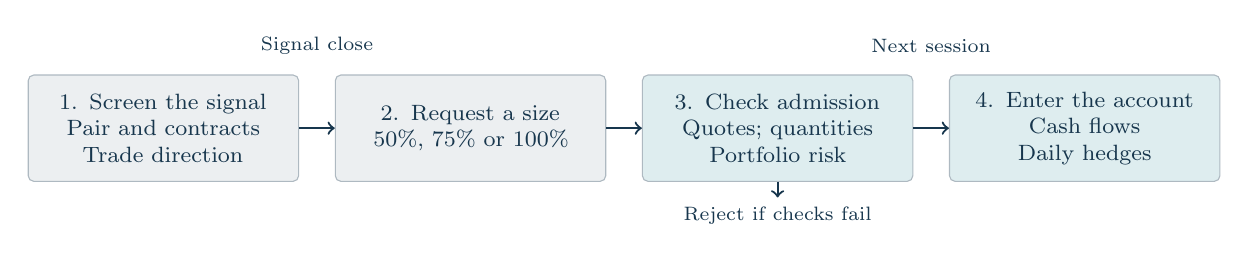
\begin{tikzpicture}[x=1cm,y=1cm,
 every node/.style={font=\footnotesize,text=navy},
 stagebox/.style={draw=navy!35,fill=navy!8,rounded corners=2pt,
 text width=3.2cm,align=center,minimum height=1.35cm},
 flow/.style={->,draw=navy,thick}]
\node[stagebox] (signal) at (1.7,0) {1. Screen the signal\\Pair and contracts\\Trade direction};
\node[stagebox] (size) at (5.6,0) {2. Request a size\\50\%, 75\% or 100\%};
\node[stagebox,fill=teal!14] (admit) at (9.5,0) {3. Check admission\\Quotes; quantities\\Portfolio risk};
\node[stagebox,fill=teal!14] (book) at (13.4,0) {4. Enter the account\\Cash flows\\Daily hedges};
\draw[flow] (signal)--(size);\draw[flow] (size)--(admit);\draw[flow] (admit)--(book);
\node[font=\scriptsize] at (3.65,1.05) {Signal close};
\node[font=\scriptsize] at (11.45,1.05) {Next session};
\draw[flow] (admit.south)--(9.5,-0.88);
\node[anchor=north,font=\scriptsize] at (9.5,-0.88) {Reject if checks fail};
\end{tikzpicture}
\caption{A signal becomes a proposal before it becomes a funded trade.
Every policy sees the same proposals; requested size and existing holdings
affect admission.}
\label{fig:workflow}
\end{figure}

Before admission, we choose quantities to approximately match initial vega: the
option-value sensitivity to a one-percentage-point IV increase.
Table~\ref{tab:trade} illustrates the entry positions at delta $-0.25$ per
share and 100 shares per contract.
\begin{table}[H]
\centering\small
\begin{tabular}{lrrl}
\toprule
Position & Contracts & Vega per IV point & Initial stock hedge\\
\midrule
Buy A puts & $+100$ & $+\money{450}$ & Buy 2,500 shares\\
Sell B puts & $-150$ & $-\money{450}$ & Short 3,750 shares\\
\bottomrule
\end{tabular}
\caption{Illustrative vega matching: A contracts have \money{4.50} vega each;
B contracts have \money{3.00}.}
\label{tab:trade}
\end{table}

After entry, hold each option to its own expiry and adjust stock delta hedges
daily. Net profit combines premiums, settlement payoffs and realized hedge
cash flows, after costs and financing. The IV rank is a hypothesis about
relative option richness. Neither initial vega matching nor temporary IV
convergence guarantees a profitable expiry outcome.

\clearpage
\subsection{Simulating trades in a funded portfolio}
\label{sec:execution}
Each policy starts with one \money{10 million} account. Historical quotes,
prices, rates and dividends come through WRDS. We inherit a 345-pair roster
and formation calendar from earlier research. Available prepared candidates
cover 125 pairs and 161 equity and ETF underlyings. After screening, 46 pairs
generate 608 proposals over 2018--2025, including 312 in the later period.
Thus, prior research and data availability condition the universe; it was not
independently selected for this comparison.

The signal selects contracts at one close; entry occurs, if eligible, at the
next session's close. We round to whole contracts and require initial vega
mismatch of at most 10\%. We then check the proposed trade alongside existing
positions. All positions share cash and capital, and stock hedges in the same
name are netted. An earlier trade can therefore prevent a new entry. Every
policy receives the same proposals, quote checks and admission rules.
Appendix~\ref{app:implementation} gives the contract and risk checks.

\begin{figure}[H]
\centering

\begin{tikzpicture}[x=1cm,y=1cm,
 every node/.style={font=\scriptsize,text=navy},
 stagebox/.style={draw=navy!35,fill=navy!8,rounded corners=2pt,
 text width=2.6cm,align=center,minimum height=1.2cm},
 flow/.style={->,draw=navy,thick}]
\node[stagebox] (carry) at (1.35,0) {1. Carry the book\\Prior positions\\and hedges};
\node[stagebox] (accrue) at (4.6,0) {2. Record accruals\\Hedge P\&L;\\dividends; funding};
\node[stagebox] (exit) at (7.85,0) {3. Settle exits\\Expiries and\\corporate events};
\node[stagebox] (entry) at (11.1,0) {4. Check entry\\Quotes and risk\\Admit if eligible};
\node[stagebox,fill=teal!14] (mark) at (14.35,0) {5. Update the book\\Rebalance hedges\\Record equity};
\draw[flow] (carry)--(accrue);\draw[flow] (accrue)--(exit);
\draw[flow] (exit)--(entry);\draw[flow] (entry)--(mark);
\end{tikzpicture}
\caption{The daily account sequence. Existing trades remain in the shared
book as new proposals arrive; the next session begins with the updated holdings.}
\label{fig:daily-account}
\end{figure}

Execution charges apply when the book trades. Options fill at midpoint, with
a charge equivalent to 0.10 IV percentage point of traded vega plus
\money{0.03} per contract. Stock hedge changes cost one basis point of turnover.
On day $t$, let $\mathcal F_t$ denote paid option fills, $\Delta n_{j,t}$ the
contracts traded in option $j$, and $V_{j,t}$ one contract's dollar vega per
IV point. For stock $s$, $P_{s,t}$ is price and $\Delta h_{s,t}$ the change in
net hedge shares. These charges give dollar execution cost
\[
C_t^{\mathrm{exec}}=\sum_{j\in\mathcal F_t}|\Delta n_{j,t}|
 (0.10V_{j,t}+0.03)+0.0001\sum_s P_{s,t}|\Delta h_{s,t}|.
\]
Expiry settlement carries no option execution charge.

Funding accrues between sessions. Short stock incurs 0.3\% annual borrow;
negative cash incurs a 1\% surcharge. Let $B_{t-1}$ be prior cash,
$H^-_{t-1}$ prior short-stock notional, and $\Delta\tau_t$ elapsed calendar
days divided by 365. Dollar funding charges are
\[
C_t^{\mathrm{fund}}=
 [0.003H^-_{t-1}+0.01\max(-B_{t-1},0)]\Delta\tau_t.
\]
Cash also earns or pays interest, $I_t=r_{t-1}B_{t-1}\Delta\tau_t$, where
$r_{t-1}$ is the prior annual benchmark rate as a decimal. Negative cash pays
both this rate and the surcharge. Appendix~\ref{app:implementation} summarizes
corporate-event exits, missing-quote handling and exercise approximations.

Finally, we compare account equity with an all-cash benchmark. This isolates
trading value after premiums, settlement, hedges, dividends, costs and financing.
Unused cash earns interest in either case, so total account growth alone does
not measure trading performance.

\clearpage
\subsection{Training, selection and testing}
We select a model specification once, then refit its tree and size map monthly.
Each fit uses historical examples from the preceding 18 months and controls
the next month's entry decisions. Figure~\ref{fig:rolling} separates these two
decisions. Training and application use successive slices of the same market history.

\begin{figure}[H]
\centering
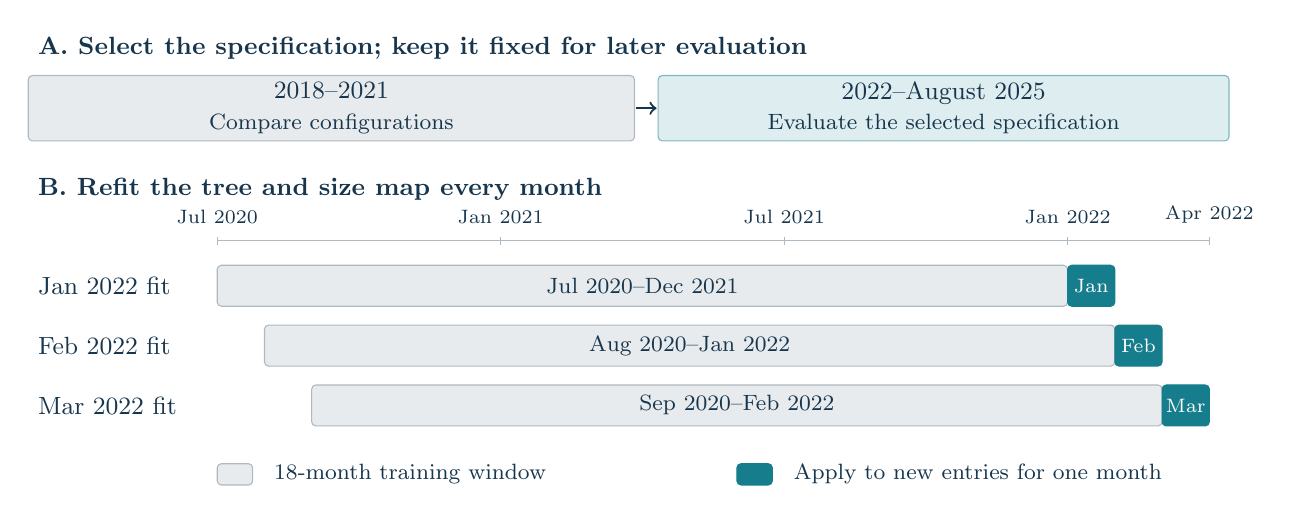
\begin{tikzpicture}[x=1cm,y=1cm,
 every node/.style={font=\small,text=navy},
 train/.style={fill=navy!10,draw=navy!35,rounded corners=1.5pt},
 apply/.style={fill=teal,draw=teal,rounded corners=1.5pt}]
\node[anchor=west,font=\small\bfseries] at (0,0)
 {A. Select the specification; keep it fixed for later evaluation};
\draw[train] (0,-1.18) rectangle (7.7,-0.35);
\node[align=center] at (3.85,-0.765)
 {2018--2021\\\footnotesize Compare configurations};
\draw[fill=teal!14,draw=teal!55,rounded corners=1.5pt]
 (8,-1.18) rectangle (15.25,-0.35);
\node[align=center] at (11.625,-0.765)
 {2022--August 2025\\\footnotesize Evaluate the selected specification};
\draw[->,draw=navy,thick] (7.72,-0.765) -- (7.98,-0.765);
\node[anchor=west,font=\small\bfseries] at (0,-1.8)
 {B. Refit the tree and size map every month};
\draw[draw=navy!35] (2.4,-2.45) -- (15,-2.45);
\foreach \x/\label in {2.4/Jul 2020,6/Jan 2021,9.6/Jul 2021,13.2/Jan 2022,15/Apr 2022}{
 \draw[draw=navy!35] (\x,-2.4) -- (\x,-2.5);
 \node[font=\scriptsize,anchor=south] at (\x,-2.35) {\label};
}
\node[anchor=west] at (0,-3.02) {Jan 2022 fit};
\draw[train] (2.4,-3.28) rectangle (13.2,-2.76);
\node[font=\footnotesize] at (7.8,-3.02) {Jul 2020--Dec 2021};
\draw[apply] (13.2,-3.28) rectangle (13.8,-2.76);
\node[text=white,font=\scriptsize] at (13.5,-3.02) {Jan};
\node[anchor=west] at (0,-3.78) {Feb 2022 fit};
\draw[train] (3,-4.04) rectangle (13.8,-3.52);
\node[font=\footnotesize] at (8.4,-3.78) {Aug 2020--Jan 2022};
\draw[apply] (13.8,-4.04) rectangle (14.4,-3.52);
\node[text=white,font=\scriptsize] at (14.1,-3.78) {Feb};
\node[anchor=west] at (0,-4.54) {Mar 2022 fit};
\draw[train] (3.6,-4.8) rectangle (14.4,-4.28);
\node[font=\footnotesize] at (9,-4.54) {Sep 2020--Feb 2022};
\draw[apply] (14.4,-4.8) rectangle (15,-4.28);
\node[text=white,font=\scriptsize] at (14.7,-4.54) {Mar};
\draw[train] (2.4,-5.55) rectangle (2.85,-5.28);
\node[anchor=west,font=\footnotesize] at (3,-5.415) {18-month training window};
\draw[apply] (9,-5.55) rectangle (9.45,-5.28);
\node[anchor=west,font=\footnotesize] at (9.6,-5.415) {Apply to new entries for one month};
\end{tikzpicture}
\caption{Two decisions, one historical dataset. The upper panel selects the
27-input, 18-month, 50/75/100\% specification using earlier performance.
The lower panel illustrates monthly refitting during evaluation. A training
example is included only if its signal date falls within the window and its
trade outcome is completed before that month's fit.}
\label{fig:rolling}
\end{figure}

For specification selection, we compare 33 existing configurations on
annualized daily excess Sharpe over 2018--2021. They vary the training history,
features and sizing actions; candidate identifiers break score ties. The
winner uses 27 inputs, an 18-month window and 50/75/100\% actions. Its selection
score is 0.575 in a \money{345 million} research account. We then replay that
configuration at \money{10 million}, using the account assumptions in
Appendix~\ref{app:implementation}.

For each monthly fit, an example must meet three conditions: it passed the
entry screens on its signal date, has a valid simulated outcome, and finished
before the fit. Its signal date must also fall within the preceding 18 months.
An example need not have been admitted to the funded account. Tree fitting
and CEM use this same sample; the profitability screens draw on the wider
candidate history.

The later comparison runs from 3 January 2022 to 29 August 2025. The selected
specification stays fixed, but monthly refitting continues. For example, a
completed March trade can inform an April fit; an unfinished outcome cannot.
New signals stop on 30 June 2025. Each account carries forward its own cash
and holdings from 2018. The 2022 boundary separates reporting periods without
resetting the accounts.

Two qualifications apply. Later history was already examined during strategy
development. Monthly fits respect time order, but the later period is not
independent of earlier contract, screen and universe choices. Training also
charges \money{0.65} commission per option contract, while final evaluation
charges \money{0.03} for every policy. We therefore interpret the comparison
as historical evidence.

\clearpage
\subsection{Learning an entry size with direct policy-search RL}
The opportunity rule has already fixed the pair, direction and contracts.
Direct policy-search RL now chooses the entry size: 50\%, 75\% or 100\% of a
reference budget of \money{450} vega per IV point on each leg. The budget
scales with current account equity relative to initial equity. To learn from
differences in historical rewards, we first group opportunities with a tree,
then choose a common size for each group (Figure~\ref{fig:tree-cem}).

Each monthly regression tree uses 27 inputs: 15 numerical characteristics and
12 availability flags. These describe relative IV, trailing realized variance,
relatedness, maturity, the CBOE Volatility Index (VIX), costs and completed
profitability; Appendix~\ref{app:features} defines them. The tree predicts
historical full-size profit above cash and chooses splits to reduce squared
prediction error. Its up to eight leaves form the states. CEM then searches
for one size to assign to each state.

\begin{figure}[H]
\centering
\setlength{\abovecaptionskip}{5pt}
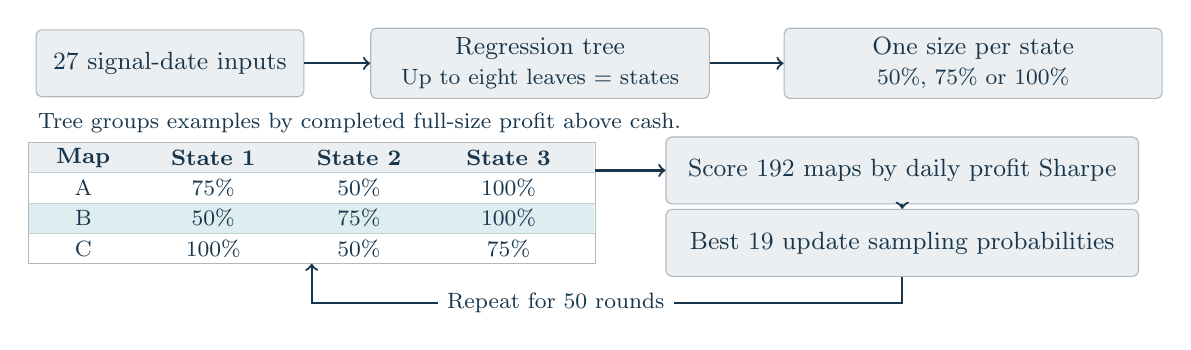
\begin{tikzpicture}[x=1cm,y=0.8cm,
 every node/.style={font=\small,text=navy},
 box/.style={draw=navy!35,fill=navy!8,rounded corners=2pt},
 flow/.style={->,draw=navy,thick}]
\node[box,align=center,minimum width=3.4cm,minimum height=0.85cm] (inputs) at (1.8,0)
 {27 signal-date inputs};
\node[box,align=center,minimum width=4.3cm,minimum height=0.85cm] (tree) at (6.5,0)
 {Regression tree\\\footnotesize Up to eight leaves = states};
\node[box,align=center,minimum width=4.8cm,minimum height=0.85cm] (map) at (12,0)
 {One size per state\\\footnotesize 50\%, 75\% or 100\%};
\draw[flow] (inputs)--(tree);\draw[flow] (tree)--(map);
\node[anchor=west,font=\footnotesize] at (0,-0.95)
 {Tree groups examples by completed full-size profit above cash.};
\draw[draw=navy!35] (0,-1.25) rectangle (7.2,-3.18);
\fill[navy!8] (0.01,-1.74) rectangle (7.19,-1.26);
\fill[teal!14] (0.01,-2.70) rectangle (7.19,-2.22);
\foreach \y in {-1.74,-2.22,-2.70}{\draw[draw=navy!25] (0,\y)--(7.2,\y);}
\foreach \x/\label in {0.7/Map,2.35/State 1,4.2/State 2,6.1/State 3}{
 \node[font=\footnotesize\bfseries] at (\x,-1.5){\label};}
\foreach \y/\name/\one/\two/\three in {-1.98/A/75/50/100,-2.46/B/50/75/100,-2.94/C/100/50/75}{
 \node[font=\footnotesize] at (0.7,\y){\name};
 \node[font=\footnotesize] at (2.35,\y){\one\%};
 \node[font=\footnotesize] at (4.2,\y){\two\%};
 \node[font=\footnotesize] at (6.1,\y){\three\%};}
\node[box,align=center,minimum width=6cm,minimum height=0.85cm] (score) at (11.1,-1.7)
 {Score 192 maps by daily profit Sharpe};
\node[box,align=center,minimum width=6cm,minimum height=0.85cm] (update) at (11.1,-2.85)
 {Best 19 update sampling probabilities};
\draw[flow] (7.2,-1.7)--(score);\draw[flow] (score)--(update);
\draw[flow] (update.south)--(11.1,-3.8)--(3.6,-3.8)--(3.6,-3.18);
\node[fill=white,font=\footnotesize] at (6.7,-3.8){Repeat for 50 rounds};
\end{tikzpicture}
\caption{Tree partitioning followed by CEM sizing search. The three-state
assignments illustrate candidate maps; actual trees have up to eight states.
The retained map applies to the next month's new proposals.}
\label{fig:tree-cem}
\end{figure}

\textbf{How CEM scores a size map}

To score a map, CEM combines completed trades' daily profit paths. Each
example has a separate path at each size, with its own rounded contracts,
standalone cash and hedge flows. These are not scaled full-size outcomes.
CEM selects paths using the map, sums them by trading day, and calculates Sharpe.

Map $\boldsymbol m$ assigns $a_\ell\in\{0.50,0.75,1.00\}$ to state $\ell$.
Example $i$ has inputs $x_i$ and state $\ell(x_i)$; $p_{i,d}(a)$ is its profit
above cash on day $d$ at size $a$. A common stored normalization cancels from
the score. Combined daily profit and training Sharpe are
\[
g_d(\boldsymbol m)=\sum_i p_{i,d}\!\left(a_{\ell(x_i)}\right),\qquad
\widehat S_{\mathrm{train}}(\boldsymbol m)=\sqrt{252}\,
\frac{\overline{g(\boldsymbol m)}}{s_{g(\boldsymbol m)}}.
\]
Here $g_d$ is combined daily profit, and the ratio uses its sample mean and
standard deviation. The factor $\sqrt{252}$ annualizes using 252 trading days.
The calendar retains overlapping trades and zero-profit sessions. This
training score uses standalone dollar profits. The funded-account Sharpe
instead uses percentage returns after joint admission checks.

CEM searches directly for a policy with a high Sharpe reward; it does not
estimate Q-values as in the motivating paper. In each of 50 rounds, it scores
192 maps and updates size probabilities toward the best 19. Constant maps
and the best map found so far remain anchors. The retained map supplies each
new proposal's requested size, which still must pass account admission.
This search does not establish a global optimum.

\clearpage
\section{Benchmark and learned-sizing results}
\subsection{Does learned entry sizing improve the benchmark?}
We first compare policies receiving the same proposals, directions and contracts.
Figure~\ref{fig:performance} plots their profit above cash. Most of the learner's
lead develops in 2022; both the learner and constant-full policy lose ground
during 2024.
\begin{figure}[H]
\centering
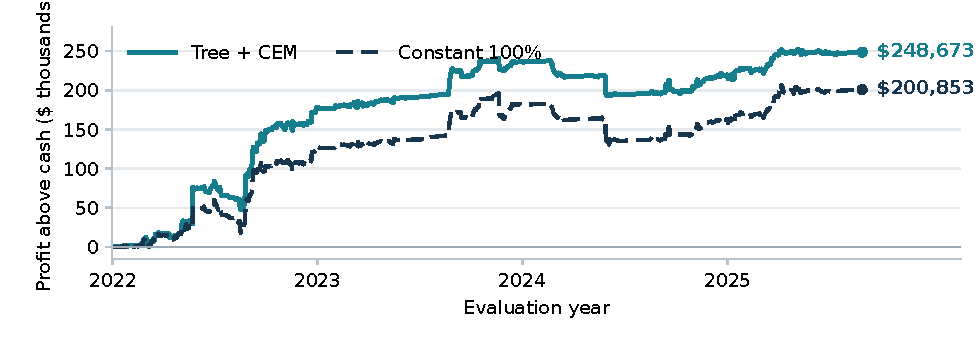
\includegraphics[width=\textwidth]{performance_above_cash.pdf}
\caption{Cumulative profit above cash, January 2022--August 2025, rebased at
31 December 2021. Accounts retain carried positions. Endpoints match
Table~\ref{tab:main}.}
\label{fig:performance}
\end{figure}

Compared with full sizing, RL raises later Sharpe by 0.208 and profit above
cash by approximately \money{47,800}. It also admits more entries: 110 versus
75. We then check rank and regression sizing, along with alternative linear
and additive RL policies that use the same training Sharpe objective.
\begin{table}[H]
\centering\small
\begin{tabular}{lrrrr}
\toprule
Policy & Earlier & Later & Later & Profit above\\
 & Sharpe & Sharpe & entries & cash (\$)\\
\midrule
Constant 50\% & 0.437 & 1.007 & 151 & 204,913\\
Constant 75\% & 0.449 & 0.944 & 104 & 195,021\\
Constant 100\% & 0.478 & 1.055 & 75 & 200,853\\
\textbf{RL: tree + CEM} & \textbf{0.573} & \textbf{1.263} & 110 & 248,673\\
\midrule
Spread-rank sizing & 0.464 & 0.815 & 121 & 164,770\\
Ridge-score sizing & 0.421 & 0.890 & 94 & 179,745\\
Direct linear policy & 0.267 & 0.873 & 96 & 171,107\\
Direct additive policy & 0.302 & 1.013 & 97 & 179,598\\
\bottomrule
\end{tabular}
\caption{Earlier: 2018--2021 replay at \money{10 million}; later:
January 2022--August 2025. The lower four rows are follow-up checks, not
original selection candidates. Earlier scores are \money{10 million}
replays, not configuration-selection scores.}
\label{tab:main}
\end{table}

Among these policies, tree/CEM has the highest funded Sharpe in both periods.
The alternatives change the sizing pipeline as a whole, not only the tree
architecture. To assess uncertainty in the later gain over full sizing, we use
a paired circular-block bootstrap with 126-session blocks and 1,000 replications.
Its interval, $[-0.103,0.424]$, includes zero and does not adjust for research search.

\subsection{Why does the admitted portfolio matter?}
To understand the result, we first sum every proposed standalone trade path
at evaluation costs. Later Sharpe is then 0.606 for tree/CEM and 0.726 for
the additive policy. Next, retain only the trades each policy's funded account
admitted. The ranking reverses: 1.268 versus 1.027, close to the funded-account
results of 1.263 versus 1.013. Smaller sizes can pass pair stress limits and
leave room for later entries. The diagnostic therefore shows an interaction
between sizing and admission. It does not isolate predictive sizing or prove
that the learner anticipated the constraints.

The learner's annualized total account return is 4.667\%, but annualized growth
relative to cash is 0.530\%. Most total growth therefore comes from interest;
trading value is measured above cash. Average reserve is 2.44\% and peak
reserve is 15.77\%. Cash-relative drawdown is 0.495\%, versus 0.646\% at full sizing.

\subsection{Variation across years and pairs}
We next examine whether the gain is spread across years and pairs.
Table~\ref{tab:annual} shows uneven annual performance. In 2024, the account
grows in total but loses relative to cash.
\begin{table}[H]
\centering\small
\begin{tabular}{lrrr@{\hspace{2em}}r}
\toprule
Year & Account return (\%) & Above cash (pp) & Excess Sharpe & Entries\\
\midrule
2022 & 3.470 & 1.673 & 2.458 & 66\\
2023 & 5.288 & 0.432 & 1.492 & 19\\
2024 & 5.104 & $-0.283$ & $-0.907$ & 11\\
2025 (partial) & 3.207 & 0.169 & 1.092 & 14\\
\bottomrule
\end{tabular}
\caption{Tree/CEM annual funded results; 2025 ends on 29 August.
Account and above-cash returns are unannualized for each displayed period,
including partial 2025. Above-cash figures are return differences in
percentage points; Sharpe is annualized.}
\label{tab:annual}
\end{table}

Profit is concentrated by pair and year. SNAP/UBER, GAP/TJX and AMD/MU
contribute 66.9\% of later net pair trading profit. Across all pairs, 2022
accounts for 83.1\% of that later profit. These percentages exclude shared
financing. They indicate concentration, rather than broad, repeated success
across pairs.

\section{Conclusion and extensions}
The retained tree/CEM RL policy improves the historical funded point estimate
over constant exposure and the tested alternative sizing pipelines. That
benefit combines exposure choices with portfolio admission. The uncertainty
interval, previously inspected history, inherited universe and simplified
execution limit what we can conclude about repeatability and live profitability.

A natural extension is to allocate across several independently researched
signals. First, freeze each signal's trade proposals. Then let RL choose
exposures using current inventory, available capital, shared underlying risks
and completed signal performance. Train against the actual funded ledger and
compare with fixed allocations. This would test whether learning can combine
opportunities into a portfolio, beyond sizing one retained signal.

\clearpage
\appendix
\footnotesize
\section{Signal and learning specification}
\label{app:implementation}
Contract selection proceeds in two steps. In the historical anchor selection,
choose the expiry closest to 30 days, then the put nearest absolute delta 0.25
within 0.075. Break ties using narrower spreads, higher open interest and
lower contract identifier. At entry, require standard 100-share contracts,
positive noncrossed quotes, open interest of at least 100, width of at most
25\% of midpoint and 7--55 days remaining. For the signal, IV rank includes
the signal close; relatedness is fixed monthly from the prior 126 sessions.
Profitability memory is dated by completion, not entry.

Admission first evaluates each name's option-plus-hedge loss under nine
combinations of spot shocks ($-20/0/+20$\%) and IV shocks ($-10/0/+10$
percentage points). Sum each name's worst loss, without credit for pair
correlation. Stress loss may not exceed 5\% of budget. Reserve, defined as
gross option premium plus half netted hedge notional, is capped at 80\%;
hedge notional is capped at twice budget. Gross vega is limited to
\money{20,000} per IV point per \money{1 million}. Global checks use account
equity; pair checks use \money{1 million} scaled by current/initial account
equity. Process proposals in pair-identifier order. These are research limits,
not broker margin requirements.

After entry, corporate events or unsupported declared distributions cause
affected pairs to exit. Missing entry quotes reject a proposal. For held
positions, marks may instead use last-known IV with current spot, rates and
known dividends. Expiry is cash-settled using a European valuation approximation.
Market impact, early assignment and forced liquidation are not fully modeled.

The tree has up to eight leaves. Its minimum leaf count is one eighth of the
training sample, rounded down and bounded between 8 and 63. With fewer than
16 examples, use full sizing. Each month, CEM starts with uniform probabilities.
For each update, mix 30\% current probability with 70\% elite frequency,
multiply by 0.97, then distribute an additional 0.03 equally across the three
actions. The random seed is 2026.

\subsection{Inputs available at the signal date}
\label{app:features}
The table defines the 15 numerical inputs. Orient proposed-direction
quantities as long leg minus short leg, and express IV and volatility levels
as decimal annualized values. To calculate trailing realized variance, take
mean squared daily simple returns over the latest 20 listed trading sessions
and multiply by 252. Require at least 10 observations and include the
signal-close return. Returns generally exclude dividends; adjusted-close
percentage changes provide the fallback series.

\begin{center}
\footnotesize
\begin{tabular}{p{0.32\textwidth}p{0.61\textwidth}}
\toprule
Input & Definition\\
\midrule
Mean IV & Mean of the two selected-contract IVs.\\
Oriented IV gap & Long-minus-short IV divided by mean IV.\\
Rank strength & Twice the absolute distance of the IV-gap percentile from 0.5.\\
Oriented variance-premium gap & Long-minus-short difference in IV squared minus trailing realized variance, divided by mean IV squared.\\
Mean RV & Mean of the square roots of the two trailing realized variances.\\
Beta; correlation & Two inputs: 126-session A-on-B beta and correlation, fixed at monthly formation.\\
Mean expiry; expiry gap & Two inputs: mean calendar days to expiry and long-minus-short expiry days.\\
Commission in IV points & Sum across legs of \money{0.65} divided by each contract's dollar vega per IV point.\\
VIX & Most recent strictly prior VIX close divided by 100.\\
91-day profit; count & Two inputs: completed full-size profit per initial vega averaged over the trailing 91 calendar days and the number of completed outcomes. The profit input is divided by 100 as a fixed scale.\\
365-day profit; count & Two inputs: the same measurements over 365 calendar days.\\
\bottomrule
\end{tabular}
\end{center}
The first three inputs are core fields. Add a binary availability flag for
each of the other 12, giving 27 inputs in total. Set a nonfinite optional
value and its flag to zero; an observed value has flag one. Profit features
use only outcomes completed before the signal date. Future returns and profits
enter the outcomes, not the inputs.

\clearpage
\section{Performance definitions and evidence}
\label{app:metrics}
We first construct the cash benchmark. Let $N_t$ be account equity and $K_t$
all-cash benchmark wealth at close $t$; both start at \money{10 million} in
January 2018. The benchmark compounds the previous available WRDS zero-curve
rate nearest 30 days over calendar days, using a 365-day year. We then subtract
its daily return from the account's daily return. This gives daily excess
return $e_t$ and annualized Sharpe
\[
e_t=\left(\frac{N_t}{N_{t-1}}-1\right)
-\left(\frac{K_t}{K_{t-1}}-1\right),\qquad
\widehat S=\sqrt{252}\,\bar e/s_e.
\]
Here $\bar e$ and $s_e$ are the sample mean and standard deviation of daily
excess returns; annualization assumes 252 trading days. For a reporting period
with preceding close $0$ and final close $T$, dollar profit above cash is the
change in excess wealth: $(N_T-K_T)-(N_0-K_0)$.

To measure growth and drawdown relative to cash, form $Q_t=N_t/K_t$.
Annualized relative growth is $(Q_T/Q_0)^{1/Y}-1$, where $Y$ is elapsed days
divided by 365.25. Cash-relative drawdown is the largest percentage decline
in $Q_t$ from its running peak within the period, including close $0$.

For the annual table, account return is $N_T/N_0-1$. Subtract benchmark
return $K_T/K_0-1$ to obtain above-cash percentage points. These period returns
are unannualized, including partial 2025; Sharpe remains annualized.

At the 31 December 2021 reporting boundary, learner equity is
\money{10.568 million} with four open trades. Constant-full equity is
\money{10.581 million} with three open trades; benchmark wealth is
\money{10.510 million}. The chart subtracts each policy's opening dollar excess
wealth. It does not reset the accounts or their holdings.

To estimate the gain interval, resample learner and constant-full daily excess
returns using identical indices. Build each of 1,000 samples by concatenating
randomly started 126-session blocks, wrapping at the series end, and truncating
to the original length. Recalculate the Sharpe difference for each sample,
then take its 2.5th and 97.5th percentiles. Fitted policies stay fixed; the
interval does not adjust for research selection.

{\raggedright
\textbf{Code and evidence in the submission.} The accompanying package contains
the main strategy implementation in \path{paper_code/} and the bundled inputs
needed to reproduce the four principal policies. Within that module,
\path{signals.py} defines screening and inputs, \path{policy.py} fits and scores
sizes, \path{ledger.py} simulates the shared account, and \path{metrics.py}
calculates performance. \path{README.md} provides setup and reproduction commands.
All paths below are relative to the package's \path{code/} directory.
The directory \path{reports/p25_validation_split} contains
\path{periods.csv}, \path{annual.csv}, \path{holdout_intervals.csv} and
\path{selection.json}. Figure~\ref{fig:performance} uses the selected account in
\path{data/p25_validation_split_experiment.zip} and the constant-full account
under \path{data/submission/artifacts/contracts/p25_capital_sensitivity}.
The complete 125-pair roster, candidate-date ranges and proposal counts are
retained in the companion \path{paper/pair_universe.csv}; ranges describe
recorded candidates, not continuous quote coverage or executed trading dates.
Inherited formation calendars and usable contracts condition the universe.
Supporting comparisons and concentration use \path{reports/p25_strategy_audit}
and \path{reports/p25_direct_policy}; the admission diagnostic is in
\path{reports/p25_generalization_bridge}.
Vendor data retain their institutional license restrictions.\par}

\begin{thebibliography}{9}
\raggedright
\bibitem{ning} B.~Ning and K.~Lee (2024).
\emph{Advanced Statistical Arbitrage with Reinforcement Learning}.
arXiv:2403.12180v1. \url{https://arxiv.org/abs/2403.12180}.
\end{thebibliography}
\end{document}

